\section{Komponenten}

%5.1 Server Software
\subsection{Komponente \textit{ServerSoftware}}
\begin{figure}[H]
\centering
\includegraphics[width=0.75\textwidth]{img/51}
\caption{\emph{ServerSoftware}-Komponentendiagramm}
\label{KomponentenStruktur1}
\end{figure}
Abbildung \ref{KomponentenStruktur1} zeigt ein Komponentendiagramm von \emph{ServerSoftware}. Diese Komponente umfasst 4 Klassen: \textit{TaskSystem}, \textit{Destination}, \textit{RobotControlSystem} und \textit{VirtualRobot}.


Das \textit{TaskSystem} verwaltet die \textit{Tasks}, in der nullten Ausbaustufe fallen dabei allerdings noch nicht viele Aufgaben an, 
da es keine Priorisierungen, unterschiedliche Arten von \textit{Tasks} oder dergleichen gibt. Die Klasse \textit{Destination} ist die Klasse 
der Aufgaben, die vom \textit{TaskSystem} verwaltet werden. Das \textit{RobotControlSystem} verteilt die \textit{Tasks} auf die \textit{Robots}. 
Dabei findet die Auswahl anhand der zurückgegebenen \textit{SensorData} der einzelnen \textit{Robots} statt. Bei \textit{VirtualRobot} handelt 
es sich um eine Kapselung der Kommunikation mit den \textit{Robots}. Hier werden alle von der Komponente \textit{Robot} bereitgestellten 
\textit{Interfaces} implementiert.
%5.1 Robot Software
\subsection{Komponente \textit{RobotSoftware}}
\begin{figure}[H]
\centering
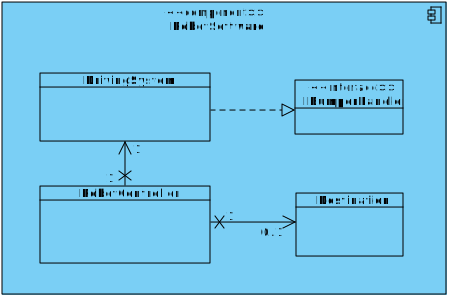
\includegraphics[width=0.85\textwidth]{img/52}
\caption{\emph{RobotSoftware}-Komponentendiagramm}
\label{KomponentenStruktur2}
\end{figure}
In Abbildung \ref{KomponentenStruktur2} ist das Komponentendiagramm der Komponente \textit{RobotSoftware} dargestellt. Sie enthält 3 Klassen: \textit{DrivingSystem}, \textit{RobotController} und \textit{Destination}. 


Das \textit{DrivingSystem} stellt eine Abstraktion der Hardware dar und wird dazu genutzt, Ziele anzufahren und dabei, 
falls nötig, Hindernisse zu umfahren. Dazu greift es auf die von der Hardware bereitgestellten \textit{Interfaces} zurück. 
Um auf Kollisionen reagieren zu können, implementiert das \textit{DrivingSystem} die Schnittstelle \textit{IBumperHandler}
Der \textit{RobotController} stellt dem Server das \emph{Interfaces} \textit{ISensorData} zur Verfügung und verwaltet den gerade 
zu absolvierenden \emph{Task} in Form einer \textit{Destination}. Zur Messwertübermittlung greift er zum einen auf das \textit{DrivingSystem} und zum anderen auf das 
von der Hardware angebotenen \textit{Interface} \textit{IBattery} zu.

